\documentclass[12pt]{article}
\usepackage[a4paper,margin=1in]{geometry}
\usepackage[T1]{fontenc}
\usepackage{textcomp}
\renewcommand{\rmdefault}{ptm}
\usepackage[scaled=0.92]{helvet}
\usepackage{mtpro2}
\usepackage[sf,bf]{titlesec}
\usepackage[font=small,width=0.7\textwidth]{caption}
\usepackage{fancybox}
\usepackage{enumerate}
\usepackage{fancyhdr}
\usepackage{rotating}
\usepackage{picins,graphicx}
\usepackage{tikz}
\usetikzlibrary{shapes,arrows}
\usepackage[pdftex]{hyperref}
\title{\sffamily\bfseries Crystallography Service Sample Database Administrator's Guide}
\author{J.P.Hagon\\Computer Systems Support\\School of Chemistry}
\date{\today}
\renewcommand{\abstractname}{Introduction}
\renewcommand{\thefootnote}{\fnsymbol{footnote}}
%
\definecolor{skyblue}{rgb}{0.422,0.648,0.801}
%
% Use these directives to change the appearance of example boxes.
%
\tikzstyle{plainbox} = [draw=blue, fill=skyblue!20, thin,
    rectangle, rounded corners, inner sep=5pt, inner ysep=5pt]
\tikzstyle{exmplbox} = [draw=blue, fill=skyblue!20, thin,
    rectangle, rounded corners, inner sep=5pt, inner ysep=15pt]
\tikzstyle{exmpltitle} =[draw=blue,fill=skyblue!50, text=white, thin]
%
% Headers
%
\pagestyle{fancy}
%
% define tikz block styles for flowcharts
%
\tikzstyle{decision} = [diamond, draw, fill=skyblue!20, 
    text width=7em, text badly centered, node distance=4cm, inner sep=0pt]
\tikzstyle{block} = [rectangle, draw, fill=skyblue!20, 
    text width=5em, text centered, rounded corners, minimum height=4em]
\tikzstyle{wideblock} = [rectangle, draw, fill=skyblue!20, 
    text width=10em, text centered, rounded corners, minimum height=4em]
\tikzstyle{line} = [draw, -latex']
\tikzstyle{cloud} = [draw, ellipse,fill=red!20, node distance=3cm,
    minimum height=2em]
%
\begin{document}
\maketitle
\begin{abstract}
This guide is intended for staff who administer the Newcastle University
Crystallography Service Sample Database.
It includes both a general description of the web interface and 
associated administration procedures along with a more technical
description of the software interface and the database itself so that
administrators can recover from situations such as a forgotton
administrator password.
\end{abstract}
\section{General Description of the System}
\subsection{Introduction}
The system consists of a \emph{front-end} which is used by users
and administrators to submit sample requests and upload analysis data. 
This front-end is implemented using the 
\href{http://www.ruby-lang.org/en/}{ruby} programming language and 
version 3 of \href{http://rubyonrails.org}{Ruby on Rails}.
The front-end is hosted on an \emph{Apache} server running on an
\emph{Ubuntu} linux system. Technical details will be described elsewhere.

The \emph{back-end} consists of a set of ruby programming libraries
and a SQL database --- in this case 
\href{http://www.sqlite.org/}{SQLite3}.
More technical aspects of the back-end will be described elsewhere.

\subsection{Users}

The system has a relatively simple user setup with just one basic user
type. However, there are three levels of authority that a user can have:
\begin{description}
\item[Standard]
Most users of the system will have a standard account which allows them
to submit sample requests and view their own sample data.
\item[Group Leader]
These users have the additional privilege of being able to see all
of the sample data for their own group in addition to their own
samples. A group of users may have more than one designated group leader.
\item[Administrator]
An administrator, in addition to standard user privileges, can do many
administration tasks. These include adding/deleting users, changing user
privileges, submitting/updating/deleting samples, editing public web
pages on the server and uploading files to the server.
\end{description}

Users can either self-register or be added by an administrator.
An administrator can also disable a user account without actually
deleting it.
Only the most basic information about a user is stored in the database,
namely first name, last name and email address. the email address serves
as a login id. The user can set his own password. If the user forgets his
password, the system can email him a secure link to the server via which
the password can be reset.

\subsection{Groups}

All users must be associated with a group. Typically this will be a
research group associated with a particular person. When a user self-registers,
he must select an appropriate group. If such a group does not exist, an
administrator must set one up for him. Usually one or more users will be
designated \emph{group leaders} and will have access to information
about all the group's samples.

\subsection{Samples}

The primary purpose of the system is to track and keep a record of
samples submitted to the crystallography service. A typical workflow is
shown in Figure \ref{fig:sample_workflow}.
Emails are sent automatically by the system when a sample status
is updated by an administrator.

\begin{figure}[!]
\small
\begin{center}
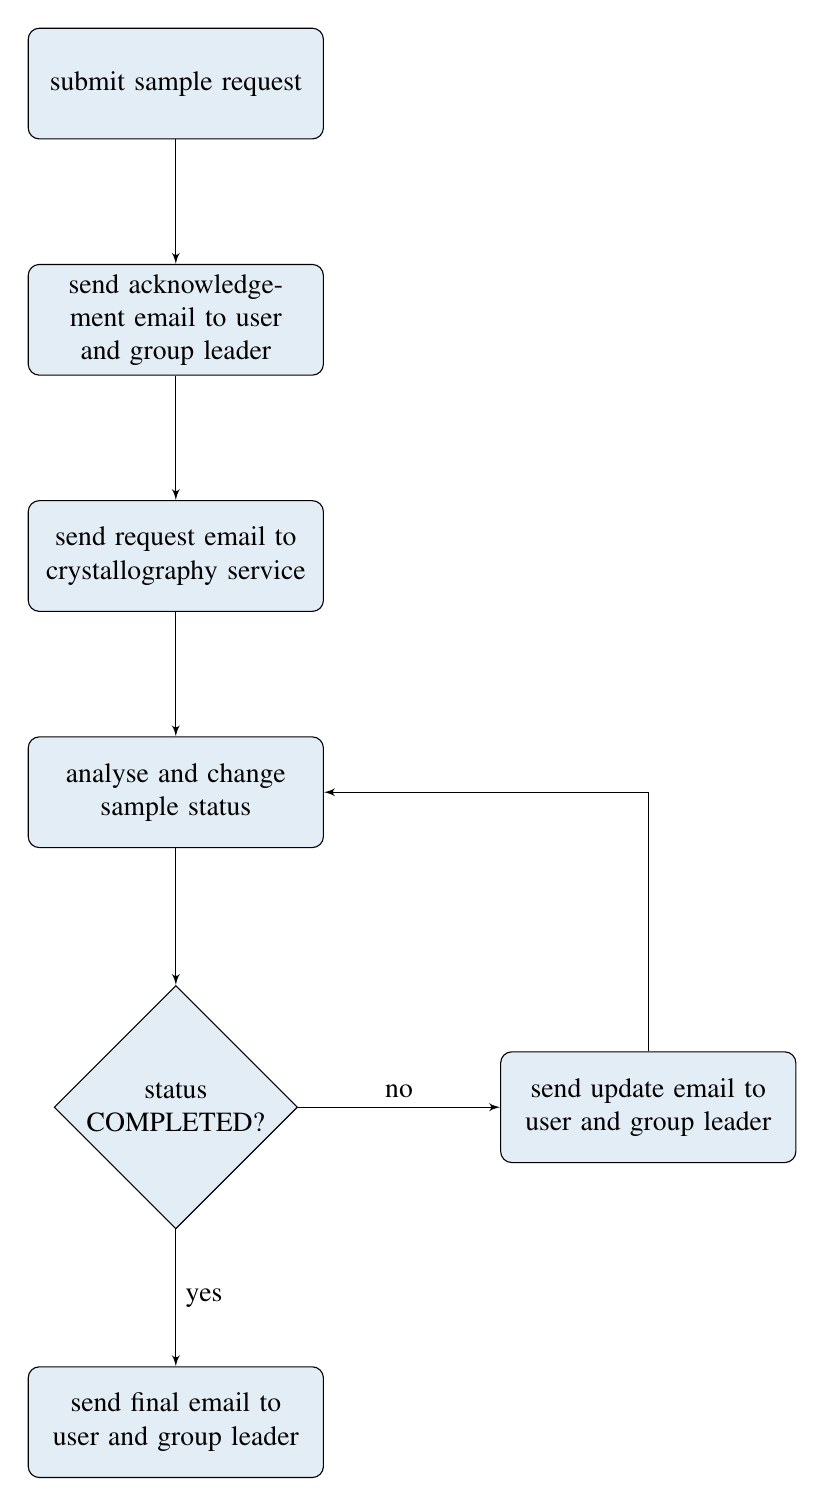
\begin{tikzpicture}[scale=2, node distance = 4cm, auto]
    % Place nodes
    \node [wideblock] (init) {submit sample request};
    \node [wideblock, below of=init, node distance=3cm] (email1) {send acknowledgement email to user
                                          and group leader};
    \node [wideblock, below of=email1, node distance=3cm] (email2) {send request email to
                                          crystallography service};
    \node [wideblock, below of=email2, node distance=3cm] (status) {analyse and change sample status};
    \node [decision, below of=status] (status1) {status\\COMPLETED?};
    \node [wideblock, right of=status1, node distance=6cm] (email4) {send update email to user
                                          and group leader};
    \node [wideblock, below of=status1] (email3) {send final email to user
                                              and group leader};
    % Draw edges
    \path [line] (init) -- (email1);
    \path [line] (email1) -- (email2);
    \path [line] (email2) -- (status);
    \path [line] (status) -- (status1);
    \path [line] (status1) -- node [, color=black] {no} (email4);
    \path [line] (status1) -- node [, color=black] {yes}(email3);
    \path [line] (email4) |- (status);
\end{tikzpicture}
\caption{Typical workflow for sample processing cycle.
Emails are sent automatically by the system whenever the status of a
sample is updated.\label{fig:sample_workflow}}
\end{center}
\normalsize
\end{figure}

\subsection{Public Pages}
Most information on the server can be viewed only by registered users.
However, there are some pages which are more generally accessible.
Such pages include the home page, general information pages and
the sample queue. Public pages can be created and edited by an administrator
using tools provided by the server software. rather than write pure
HTML, an administrator can use a text-based markup language called
\href{http://en.wikipedia.org/wiki/Textile_%28markup_language%29}{Textile}
which can produce sophisticated web pages with all the usual constructs
such as headings, paragraphs, floating elements, tables and images.

\section{Web Management Guide}
\subsection{Introduction}
In this section we describe the web management interface to the
sample tracking database. When a manager is logged-in, the home page of
the system looks similar to that shown in Figure \ref{fig:homepage}

\begin{figure}[!h]
\begin{center}
\includegraphics[width=0.75\textwidth]{homepage}
\caption{Administrator's view of home page.\label{fig:homepage}}
\end{center}
\end{figure}

There are three parts to this browser view:
\begin{enumerate}[(i)]
\item
a main display showing the contents of a page of information;
\item
a menu on the left side of the browser window;
\item
login information and a \verb=sign_out= link above the main display on
the right.
\end{enumerate}

The left side menu consists of three sections:
\begin{description}
\item[Information]
These links point to \emph{static} pages which can be created by an
administrator. the administrator can also add extra links to the
information section. We describe how to do this in \S\ref{sec:static}.
\item[User Tools]
These tools allow a user to view his sample list, submit a new sample
and view his profile information. Additionally, if a user is also a group
leader, he will have access to the \emph{My Group Samples} link for listing
all samples in the user's group.
\item[Admin Tools]
This is the main set of web-based tools for administrators. We will
describe each of these in the next section.
\end{description}
\subsection{Adding Static Pages}\label{sec:static}
Clicking the \emph{PAGES} link in the \emph{Admin Tools} sub-menu 
produces the pages index shown in Figure \ref{fig:pageidx}.
This shows a list of pages. For each of these pages is a set of buttons
allowing the administrator to show, edit or delete the page as shown in
Figure \ref{fig:showeditdelete}.
These buttons are used throughout the database editing pages on the web server.
At the bottom of the list is a link to create a new page.

\begin{figure}[!h]
\begin{center}
\includegraphics{show}\quad
\includegraphics{edit}\quad
\includegraphics{delete}
\end{center}
\caption{The \emph{show}, \emph{edit} and \emph{delete} buttons.
\label{fig:showeditdelete}}
\end{figure}

\begin{figure}[!h]
\begin{center}
\includegraphics[width=0.75\textwidth]{pageidx}
\caption{The pages index view.\label{fig:pageidx}}
\end{center}
\end{figure}

\piccaption{The page edit view.\label{fig:editpage}}
\parpic[r]{\includegraphics[width=0.4\textwidth]{editpage}}
Figure \ref{fig:editpage} shows the page editor --- a very simple form
for entering/changing text. This example shows the home page data. 
the content is entered in a markup language called Textile\footnote{You are 
allowed to mix HTML and Textile together.}. You can also specify the name
of the page (this will be used to set the HTML title attribute and a
permalink\footnote{A tag which is used as a basis for a concise URL.}.
At the bottom are links to the Textile Reference Manual, the page view
and the pages index. the page can be referred to via the URL:
\begin{verbatim}
<server name>/permalink
\end{verbatim}
thus making static page addressing very simple.
An alternative URL which can be generally used for any page is:
\begin{verbatim}
<server name>/pages/<id>
\end{verbatim}
but the permalink-based URL is what you'd almost always use in practice.
If, for some reason, you want to use the id-based URL, but don't know
what the id is, then just click the 'show' icon in the pages index for
the page you're interested in and look at the URL in the web browser window.

Note that there is also a checkbox labelled \emph{Menu}. If this is
checked then the page is added to the left hand \emph{Information} menu
of static pages. The \emph{Priority} parameter is an integer that
determines the order of the page in the menu. If two pages have the same
priority their order is determined alphabetically.

\subsection{Uploading General Files to the Server}
You can upload arbitrary files to the server. These files are referred
to as `assets' and can be uploaded via the \emph{ASSETS} link in the
\emph{Admin Tools} menu. Clicking on this link will take you to the
assets index page which looks very similar to the pages index described
in the previous section.
each index entry tells you the pathname of the file on the server,
together with a description of what the file contains. Often these files
will be images or documents (e.g. PDF files) that you want to link to
on one of the static web pages created as described in the previous
section.

At the bottom of the asset index list is a link to create a new asset.
Clicking this takes you to a simple menu where you can browse for a file
to upload to the server. Clicking the \emph{Create Asset} button will
then upload the file to the server. It will then be listed in the
asset index with an entry under the \emph{Document} column pointing
to its location in the file system. This location has the general form:
\begin{verbatim}
/uploads/asset/document/<id>/<filename>
\end{verbatim}
Here, \verb=<filename>= is the actual name of the uploaded file as it was
when it was uploaded. \verb=<id>= is the database id the document has
in the \verb=assets= table described in detail in \S\ref{sec:database}.
The actual URL of the document is then:
\begin{verbatim}
<servername>/uploads/asset/document/<id>/<filename>
\end{verbatim}

\subsection{Creating Users and Groups}
A user must belong to a group, so it is advisable to create a group for a
user before the user is created. Creating a user group is straightforward
via the \emph{USER GROUPS} link in the \emph{Admin Tools} menu.
As usual, this will take you to an index of existing groups, with a link
to create a new group at the bottom. Creating a new group merely requires
that you enter two fields:
\begin{enumerate}[(i)]
\item
a 3-letter group abbreviation (it \emph{must} be three letters);
\item
a longer group description.
\end{enumerate}

Users can be created in two ways; they can self-register by clicking
on the link top-right on the home page or they can be created by an
administrator. In either case the form used to create and register a new
user is the same.


\section{The Database}\label{sec:database}
\subsection{Introduction}
The core of the system is the database which holds information about 
users, samples etc. In this section we describe the whole database
structure (or \emph{schema} in database parlance).
The easiest way to get an overall view of the database schema is to
study Figure \ref{fig:database_schema}. This shows
all the tables, fields and relationships in a single diagram.
We now give a brief description of each table.

Note that all tables except join tables have an autoincremented integer field
called \verb=id= which servers as the unique primary key for each record
in the table. The \verb=id= field will not be listed explicitly in the
description of each table. All non-join tables also have two other
fields, \verb=created_at= and \verb=updated_at= in a datetime format.
Again, we will not explicitly list these fields in the description
of the tables which follows.

\subsection{The Samples Table}
The samples and users tables are the key parts of the database as is
evident from Figure \ref{fig:database_schema}. They are related to each
other via a \emph{one-to-many} relationship, i.e. \emph{one} user
can have \emph{many} samples. The samples table
consists of the following fields:
\begin{description}
\item[code]
a string, automatically generated by the system having the
general form \verb=AAA-AA-YY-1111= where the \verb=AAA= and \verb=AA= 
represent 3-letter codes for group and submitter respectively; 
the \verb=YY= represents the year and the \verb=1111= represents a number 
which is incremented for that group but reset to zero at the start of each 
calendar year.
\item[cif]
a string representing the chemical formula of the sample in cif format.
\item[synth]
a string representing the file name of an image file specifying the details
of the synthesis.
\item[coshh\_name]
a string representing the name of the solvent (if any).
\item[coshh\_info]
another string describing any procedures in case of contact with the sample.
\item[coshh\_desc]
a text field providing a brief description of the sample (e.g. organic amide).
\item[params]
a string representing unit cell parameters
or CSD/Newcastle code for possible by-products or previously obtained, 
unpublished results.
\item[priority]
an integer between 1 and 9 to give an indication of priority.
\item[powd]
a boolean parameter indicating if the sample requires powder diffraction (y/n).
\item[chiral]
another boolean indicating whether the molecule is chiral (y/n).
\item[costcode]
a string providing a cost centre code for charging if relevant.
\item[barcode]
a string field for an automatically generated Code39 standard barcode.
\item[user\_id]
this integer holds the \verb=id= field of the user who requested the
sample analysis.
\item[flag\_id]
an integer holding the \verb=id= field of the status flag of the sample.
\item[userref]
a string for a user-defined reference. This is required to be an
alphanumeric sequence of characters \emph{without spaces}.
\item[zipdata]
a string holding the name of a zipfile containing the results of the analysis.
\item[sampleimage]
a string holding the name of an image file of the sample molecule after it
has been identified by the analysis.
\item[reference]
a text field for a published reference (typically in the form of a DOI).
\item[comments]
a text field for any general comments the user wishes to make about the sample.
\item[colour]
a string holding information about the colour of a sample after analysis.
\item[size]
a string holding information about the size of a sample after analysis.
\item[shape]
a string holding information about the shape of a sample after analysis.
\end{description}

\subsection{The Users Table}
The users table, in addition to maintaining a record of users and their
samples, also serves as a key part of the authentication and authorization
system which will be described later. the users table is related to the
samples table via a \emph{one-to-many} relationship, i.e. \emph{one} user
has \emph{many} samples.
\begin{description}
\item[email]
a string holding the email address of the user. This serves also as the
user login id.
\item[encrypted\_password]
a string holding the user's password in an encrypted form.
\item[reset\_password\_token]
a string containing a special token used if the user has forgotten his
password and needs to reset it.
\item[reset\_password\_sent\_at]
a datetime field recording the time a token enabling a user to reset his
password was sent.
\item[remember\_created\_at]
a datetime field specifying the time at which a user requested that his
login id be remembered by the browser so he need not type in his credentials.
\item[sign\_in\_count]
an integer holding the number of times a user has logged-in.
\item[current\_sign\_in\_at]
a datetime field holding the sign-in time for the current session.
\item[last\_sign\_in\_at]
a datetime field holding the last sign-in time for the user.
\item[current\_sign\_in\_ip]
a datetime field holding the user's ip address for the current session.
\item[last\_sign\_in\_ip]
a datetime field holding the previous login ip address for the user.
\item[group\_id]
an integer representing the \verb=id= field of the group to which
the user belongs.
\item[admin]
a boolean field indicating whether the user is an administrator (y/n).
\item[firstname]
a string holding the user's first name.
\item[lastname]
a string holding the user's last name.
\item[leader]
a boolean field indicating whether the user is a group leader (y/n).
\item[enabled]
a boolean field indicating if the account is enabled (y/n).

\end{description}

\subsection{The Stores, Hazards and Sensitivities Tables}
These tables are each very similar and have the same basic structure.
They are used to specify storage, hazard and sensitivity properties
for a sample. They all have a \emph{many-to-many} relationship with
the samples table. This is because a sample can have, for example,
\emph{many} storage requirements, but also a single storage requirement
can be associated with \emph{many} samples.
All these tables have essentially the same fields:
\begin{description}
\item[name]
a string defining a short name for the property.
\item[description]
a text field describing the property at greater length.
\end{description}
For historical reasons, the hazards table uses the names
\verb=hazard_abbr= and \verb=hazard_desc= for the \verb=name= and
\verb=description= fields. Also the \verb=hazard\_desc= field is a text
field rather than a string.

Associated with these tables are three further \emph{join tables} which
facilitate the many-to-many relationship between a sample and its
properties. These join tables are called \verb=samples_stores=,
\verb=samples_hazards= and \verb=samples_sensitivities=. They all contain
two fields corresponding to the sample \verb=id= field and the associated
property \verb=id= field. For example, \verb=samples_stores= contains the
fields \verb=sample_id= and \verb=store_id=. Both these fields are integers
of course.

\subsection{The Groups Table}
This table represents groups of users, normally research groups but also
perhaps external companies etc.
It is a simple table, but important in the way the whole system works.
It contains the following fields:

\begin{description}
\item[group\_abbr]
a 3-letter string as an abbreviation for the group. Amongst other things
this is used to form part of the sample code string mentioned earlier.
\item[group\_desc]
a string giving a more complete description of the group.
\end{description}

\subsection{Other Tables}
There are several other tables which are less important than the ones 
discussed so far in the sense that they are strictly not necessary for
a working sample tracking system. However, they do assist in making the
system much easier to manage and also help making the system much
friendlier for users. These tables are the \verb=assets=, \verb=pages=
and \verb=popups= tables.

\subsubsection{The Pages Table}
The purpose of this table is to provide a means by which administrators can
add `static' content to the sample tracking web site. Each static page has
its content stored in this table. The fields are:

\begin{description}
\item[name]
a string storing a name for the page. This is typically used to provide
a title for the page in a web browser window.
\item[permalink]
another string used to provide a short, quick URL for the page.
\item[content]
a text field which contains the page content. This is expected to be written
in  \href{http://en.wikipedia.org/wiki/Textile_%28markup_language%29}{Textile}
markup language (although a mixture of pure HTML and Textile can be used.
\item[menu]
a boolean specifying whether this page should appear on the
\emph{Information Menu}.
\item[priority]
an integer specifying a priority for ordering the page on the
\emph{Information Menu}.
\end{description}

\subsubsection{The Assets Table}
The assets table keeps a record of general files which have been uploaded
to the server. These files are typically graphical images, pdf documents etc.
and will usually be referenced in one of the static pages created by
administrators which are stored in the \verb=pages= table. An `asset' is
simply one of these uploaded documents and the \verb=assets= table keeps
a record of it. The fields are:

\begin{description}
\item[document]
the full path name of an uploaded document. This path name is ultimately
assigned using the 
\href{https://github.com/jnicklas/carrierwave}{carrierwave}
file uploading plugin to ruby on rails.
\item[description]
a text field giving a brief description of the document.
\end{description}

\subsubsection{The Popups Table}
This table stores descriptive information about the primary fields
in the samples table. It has two fields:

\begin{description}
\item[name]
this string should have the same name as one of the sample fields for
which a detailed description is required.
\item[description]
a text field giving a detailed description of the associated sample field
in the corresponding \verb=name= field.
\end{description}

The \verb=popups= table, as its name implies, provides descriptive
text in popup boxes whenever a user hovers the mouse over the
appropriate field in the sample submission form.

\begin{sidewaysfigure}
\captionsetup{width=25cm}
\begin{center}
\pgfdeclarelayer{background}
\pgfsetlayers{background,main}
\begin{tikzpicture}[every text node part/.style={text centered}, font=\small]
\tikzset{every node/.style={rectangle split, 
                            rectangle split parts=2, 
                            draw, text width=3.5cm}}

\node(assets) [rectangle split part fill={skyblue!20, white}]
  {ASSETS
  \nodepart{second}
  id:int \\
  document:string \\
  description:text \\
  created\_at: datetime \\
  updated\_at: datetime};

\node(pages) [below of=assets, node distance=4cm, 
              rectangle split part fill={skyblue!20, white}]
  {PAGES
  \nodepart{second}
  id:int \\
  name:string \\
  permalink:string \\
  content:text \\
  menu:boolean \\
  priority:int \\
  created\_at: datetime \\
  updated\_at: datetime};

\node(popups) [below of=pages, node distance=4cm,  
               rectangle split part fill={skyblue!20, white}]
  {POPUPS
  \nodepart{second}
  id:int \\
  name:string \\
  description:text \\
  created\_at: datetime \\
  updated\_at: datetime};

\node(groups) [below of=popups, node distance=4cm,
               rectangle split part fill={skyblue!20, white}]
  {GROUPS
  \nodepart{second}
  id:int \\
  group\_abbr:string \\
  group\_desc:string \\
  created\_at: datetime \\
  updated\_at: datetime};

\node(users) [left of=popups, node distance=5cm,
               rectangle split part fill={skyblue!20, white}]
  {USERS
  \nodepart{second}
  id:int \\
  email:string \\
  {\scriptsize encrypted\_password:string} \\
  {\scriptsize reset\_password\_token:string} \\
  {\tiny reset\_password\_sent\_at:datetime} \\
  {\tiny remember\_created\_at: datetime} \\
  sign\_in\_count:int \\
  {\scriptsize current\_sign\_in\_at:datetime} \\
  {\scriptsize last\_sign\_in\_at:datetime} \\
  {\scriptsize current\_sign\_in\_ip:datetime} \\
  {\scriptsize last\_sign\_in\_ip:datetime} \\
  created\_at: datetime \\
  updated\_at: datetime \\
  group\_id:int \\
  admin:boolean \\
  firstname:string \\
  lastname:string \\
  leader:boolean \\
  enabled: boolean};

\node(samples) [left of=users, node distance=5cm,
               rectangle split part fill={skyblue!20, white}]
  {SAMPLES
  \nodepart{second}
  id:int \\
  code:string \\
  cif:string \\
  synth:string \\
  synth:string \\
  coshh\_name:string \\
  coshh\_info:string \\
  coshh\_desc:text \\
  params:string \\
  priority:int \\
  powd:boolean \\
  chiral:boolean \\
  costcode:string \\
  barcode:string \\
  created\_at: datetime \\
  updated\_at: datetime \\
  user\_id:int \\
  flag\_id:int \\
  userref:string \\
  zipdata:string \\
  sampleimage:string \\
  reference:string \\
  comments:text \\
  colour:string \\
  size:string \\
  shape:string };

\node(sampsen) [left of=samples, node distance=5cm,
               rectangle split part fill={skyblue!20, white}]
  {{\scriptsize SAMPLES\_SENSITIVITIES}
  \nodepart{second}
  sample\_id:int \\
  sensitivity\_id:int};


\node(samphaz) [above of=sampsen, node distance=4cm,
               rectangle split part fill={skyblue!20, white}]
  {{\footnotesize SAMPLES\_HAZARDS}
  \nodepart{second}
  sample\_id:int \\
  hazard\_id:int};

\node(sampsto) [above of=samphaz, node distance=4cm,
               rectangle split part fill={skyblue!20, white}]
  {{\footnotesize SAMPLES\_STORES}
  \nodepart{second}
  sample\_id:int \\
  store\_id:int};

\node(sensitivities) [left of=sampsen, node distance=5cm,
               rectangle split part fill={skyblue!20, white}]
  {SENSITIVITIES
  \nodepart{second}
  id:int \\
  name:string \\
  description:text \\
  created\_at: datetime \\
  updated\_at: datetime};

\node(flags) [below of=sensitivities, node distance=4cm,
               rectangle split part fill={skyblue!20, white}]
  {FLAGS
  \nodepart{second}
  id:int \\
  name:string \\
  description:text \\
  created\_at: datetime \\
  updated\_at: datetime};


\node(hazards) [above of=sensitivities, node distance=4cm,
               rectangle split part fill={skyblue!20, white}]
  {HAZARDS
  \nodepart{second}
  id:int \\
  hazard\_desc:string \\
  hazard\_abbr:string \\
  created\_at: datetime \\
  updated\_at: datetime};

\node(stores) [above of=hazards, node distance=4cm,
               rectangle split part fill={skyblue!20, white}]
  {STORES
  \nodepart{second}
  id:int \\
  name:string \\
  description:text \\
  created\_at: datetime \\
  updated\_at: datetime};

\coordinate[below=0.6em] (sampleid-w) at (samples.text split west);
\coordinate[below=0.6em] (sampleid-e) at (samples.text split east);
\coordinate[below=0.6em] (userid-w) at (users.text split west);
\coordinate[below=0.6em] (groupid-w) at (groups.text split west);
\coordinate[below=0.6em] (storeid-e) at (stores.text split east);
\coordinate[below=0.6em] (hazardid-e) at (hazards.text split east);
\coordinate[below=0.6em] (sensitivityid-e) at (sensitivities.text split east);
\coordinate[below=0.6em] (flagid-e) at (flags.text split east);

\coordinate[below=20em] (samples-flagid-w) at (samples.text split west);
\coordinate[below=19em] (samples-userid-e) at (samples.text split east);

\coordinate[below=15.5em] (users-groupid-e) at (users.text split east);

\coordinate[below=0.6em] (sampsto-sampid-e) at (sampsto.text split east);
\coordinate[below=0.6em] (samphaz-sampid-e) at (samphaz.text split east);
\coordinate[below=0.6em] (sampsen-sampid-e) at (sampsen.text split east);

\coordinate[above=0.6em] (sampsto-stoid-w) at (sampsto.south west);
\coordinate[above=0.6em] (samphaz-hazid-w) at (samphaz.south west);
\coordinate[above=0.6em] (sampsen-senid-w) at (sampsen.south west);

\begin{pgfonlayer}{background}

  \tikzstyle{line} = [draw]
  \path [line] (sampsto-sampid-e) -- (sampleid-w);
  \path [line] (samphaz-sampid-e) -- (sampleid-w);
  \path [line] (sampsen-sampid-e) -- (sampleid-w);

  \path [line] (sampsto-stoid-w) -- (storeid-e);
  \path [line] (samphaz-hazid-w) -- (hazardid-e);
  \path [line] (sampsen-senid-w) -- (sensitivityid-e);

  \path [line] (flagid-e) -- (samples-flagid-w);

  \path [line] (samples-userid-e) -- (userid-w);

  \path [line] (users-groupid-e) -- (groupid-w);

\end{pgfonlayer}

\end{tikzpicture}
\end{center}
\caption{The overall database schema. Relationships between tables are
indicated with lines joining the relevant fields. Note that the tables
\texttt{SAMPLES\_STORES}, \texttt{SAMPLES\_HAZARDS} and 
\texttt{SAMPLES\_SENSITIVITIES}
are \emph{join tables} which serve only to facilitate a many-to-many
relationship between the tables they link.\label{fig:database_schema}}
\end{sidewaysfigure}
\newpage
\tableofcontents
\newpage
\end{document}
